%%%%%%%%%%%%%%%%%%%%%%%%%%%%%%%%%%%%%%%%%%%%%%%%%%%%%%%%%%%%%%%%%%%%%%%%%%%%%%%%%%%%%%%%%%%%%
%%									Chapitre 6												%
%%%%%%%%%%%%%%%%%%%%%%%%%%%%%%%%%%%%%%%%%%%%%%%%%%%%%%%%%%%%%%%%%%%%%%%%%%%%%%%%%%%%%%%%%%%%%

\chapter{Perspectives}
	\minitoc

%%%%%%%%%%%%%%%%%%%%%%%%%%%%%%%%%%%%%%%%%%%%%%%%%%%%%%%%%%%%%%%%%%%%%%%%%%%%%%%%%%%%%%%%%%%%%

Le protocole mis en place dans le cadre de cette thèse permet de définir un premier
environnement autorisant la modélisation des flux intracrâniens sujet-spécifique. L’acquisition et le
traitement des images sont suffisamment génériques pour permettre d’une part d’intégrer les
nouvelles versions des séquences et d’autres part développer le modèle avec les avancées techniques.
L’intégration des différentes modalités d’imagerie peut se faire à plusieurs niveaux. La carte de
susceptibilité magnétique par exemple fournit une information plus précise sur les petites structures
veineuses en comparaison du contraste de phase et de de la simple SWI. De même l’ASL assure un
ajustement des résistances pour certains compartiments (capillaires etc.) et permet de contrôler les
écarts entre le modèle et la réalité. Cependant la QSM fournit en plus une information sur la saturation
veineuse en oxygène dans les veines, reflétant directement la consommation dans le lit capillaire, on
associe ainsi un territoire capillaire à sa saturation en oxygène. Ce n’est pas une donnée directement
intégrée dans la simulation, elle apporte cependant une information supplémentaire caractérisant les
compartiments. Associée à l’imagerie ASL via un protocole particulier, il devient possible d’estimer la
consommation moyenne en oxygène (CMRO2) (\cite{Zhang2014}).

Le développement de nouvelles séquences IRM permet d’atteindre des résolutions beaucoup
plus fines avec de meilleurs contrastes. Le modèle, tel qu’il est généré s’adapte à cet apport
supplémentaire d’information ce qui le rend plus détaillé. Cependant, les plus petits vaisseaux restent
très difficiles à imager. Il est peu probable qu’à court terme, une séquence d’IRM sans injection arrive
à fournir suffisamment de détails pour appréhender très précisément l’ensemble de l’arbre vasculaire.
C’est pourquoi de nouvelles approches se développent, nommées « Constructive Optimization ». Le
principe est de déterminer le réseau vasculaire répondant à un critère d’optimalité physiologique (par
exemple minimisant le volume intravasculaire) pour une exigence d’alimentation donnée (\cite{Schwen2012}). Les
« Constrained Constructive Optimization » (CCO) représentent l’approche prédominante (\cite{Schreiner1993},~\cite{Karch1998}),
elle consiste à retrouver dans un espace convexe fournit (par exemple le crâne) l’arborisation
vasculaire optimale. Cet outil a été principalement utilisé sur le foie où la vascularisation est très
caractérisée  (\cite{Georg2010}, Figure~\ref{fig:7_1_arbos}). On construit un arbre binaire en ajoutant un nœud terminal à chaque
temps à un arbre initial, chaque temps introduisant une bifurcation optimale. Les CCO peuvent être vu
comme étant dirigé par l’hypothèse d’égalité des flux entrants ou sortants de chaque nœud terminal.
De plus, aux bifurcations, les rayons sont équilibrés de telle façon à ce que la résistance selon la loi de
Hagen-Poiseuille soit égale dans les deux sous-arbres. Il en résulte des pressions égales aux sorties des
nœuds terminaux.

%%%
\begin{figure}[!t]
\centering
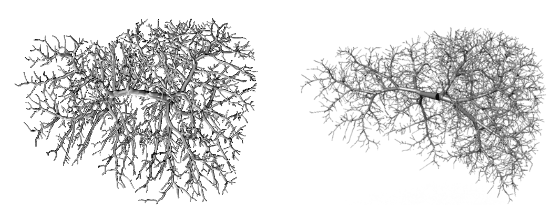
\includegraphics[width=9cm]{7_1_arbos}
\caption{Résultats obtenus par Georg et al. (\cite{Georg2010}) sur le foie par utilisation de CCO. A gauche un arbre vasculaire obtenu in
vitro par « corrosion cast imaging » (\cite{Hahn2003}). A droite les résultats d’une simulation du système vasculaire du foie sur la base
d’images de scanner.}
\label{fig:7_1_arbos}	
\end{figure}
L’intérêt de ce genre d’approche est qu’elles peuvent être guidées par des cartographies annexes en
vue d’optimiser la structure vasculaire. Il est donc tout à fait envisageable à partir de notre protocole
de se servir des données de débit issue de l’ASL pour guider ce genre d’algorithme et aboutir à une
représentation plausible d’une partie importante de la vascularisation.

Les prochains développements du modèle devront donc l’enrichir de données morphologiques
plus précises grâce aux évolutions des séquences, mais aussi aux CCO. Une meilleure intégration des
données physiologiques assurera par ailleurs une fidélité importante du modèle à la réalité.

Il est enfin important de valider le modèle sur des cohortes plus importantes pour s’assurer de sa reproductibilité. 







\bibliography{jeremythesebib}{}
\bibliographystyle{francaissc}